%%%% ijcai19-multiauthor.tex

\typeout{IJCAI-19 Multiple authors example}

% These are the instructions for authors for IJCAI-19.

\documentclass{article}
\pdfpagewidth=8.5in
\pdfpageheight=11in
% The file ijcai19.sty is NOT the same than previous years'
\usepackage{ijcai19}

% Use the postscript times font!
\usepackage{times}
\usepackage{soul}
\usepackage{url}
\usepackage[hidelinks]{hyperref}
\usepackage[utf8]{inputenc}
\usepackage[small]{caption}
\usepackage{amsmath}
\usepackage{booktabs}
\urlstyle{same}
%%
% FIGURES
\usepackage{graphicx}
\graphicspath{./figs}
\usepackage{grffile} % to set right names of files
%%
% CAPTIONS
\usepackage{caption}
\usepackage{subcaption} % supersedes subfigure & subfloat. try using options
%%
% LISTS
\usepackage{enumitem} %\begin{itemize}[leftmargin=*]
%% inline
\newlist{inline}{enumerate*}{1}
\setlist[inline]{before=\unskip{: }, itemjoin={{; }}, itemjoin*={{; and }}, label={(\roman*)}}
\usepackage{silence}
\WarningFilter{ctable}{Transparency disabled:}
\WarningFilter{xcolor}{Incompatible color}

% the following package is optional:
%\usepackage{latexsym} 

% Following comment is from ijcai97-submit.tex:
% The preparation of these files was supported by Schlumberger Palo Alto
% Research, AT\&T Bell Laboratories, and Morgan Kaufmann Publishers.
% Shirley Jowell, of Morgan Kaufmann Publishers, and Peter F.
% Patel-Schneider, of AT\&T Bell Laboratories collaborated on their
% preparation.

% These instructions can be modified and used in other conferences as long
% as credit to the authors and supporting agencies is retained, this notice
% is not changed, and further modification or reuse is not restricted.
% Neither Shirley Jowell nor Peter F. Patel-Schneider can be listed as
% contacts for providing assistance without their prior permission.

% To use for other conferences, change references to files and the
% conference appropriate and use other authors, contacts, publishers, and
% organizations.
% Also change the deadline and address for returning papers and the length and
% page charge instructions.
% Put where the files are available in the appropriate places.

\title{Interpreting Complex System Dynamics Under Data Scarcity: An
Application to Invasive Species Spread}

%% \author{
%% First Author$^1$\footnote{Contact Author}\and
%% Second Author$^2$\and
%% Third Author$^{2,3}$\And
%% Fourth Author$^4$\\
%% \affiliations
%% $^1$First Affiliation\\
%% $^2$Second Affiliation\\
%% $^3$Third Affiliation\\
%% $^4$Fourth Affiliation\\
%% \emails
%% \{first, second\}@example.com,
%% third@other.example.com,
%% fourth@example.com
%% }

\begin{document}

\maketitle

\begin{abstract}
Networked agent-based models are being increasingly used to study spread of
diseases and invasive species. However, data scarcity coupled with
complexity of the model can lead to multiple explanations for the observed
phenomenon; simulation outputs very different from one another can closely
match the ground truth. Delimiting configuration subspaces that lead to
such variability helps identify knowledge gaps, and therefore guide data
collection and policy making. We present a novel framework to analyze
complex simulation systems using machine learning tools. It is applied to
the study of an invasive pest of tomato crop that has spread globally in
the last decade threatening food security and social welfare. Simulated
spread patterns are clustered to capture variability. The resulting
clusters are further analyzed using decision trees to discover relationship
with model parameters. This work touches two emerging topics in a novel
way: machine learning aided simulation systems, and explainable AI.
\end{abstract}

\section{Introduction}
\paragraph{invasive species} standard stuff on invasive species: afri, bigdata, complex networks
UN stuff

\paragraph{complexity of the phenomenon} 
multiple pathways: natural factors, self-mediated spread, human-mediated spread
what is a policy maker looking for

\paragraph{ABMs and ML in IAS.}
mainly ML has been used for ecological suitability
ABMs used for seed dispersal, human-mediated, seed networks ...
Garrett, Rebaudo, etc. to be just referred to
Here we focus mainly on ABMs.

\paragraph{Challenges} try old naturecomm. 
inaccuracies in incidence, particularly emerging
diseases. we don't know how the pest behaves. basically, data and model
uncertainty.

overfitting
high-resolution


\section{Methodological framework}
\paragraph{description with notation}

\paragraph{an illustrative example}

\section{Application}
%%
\begin{figure}[t]
\centering
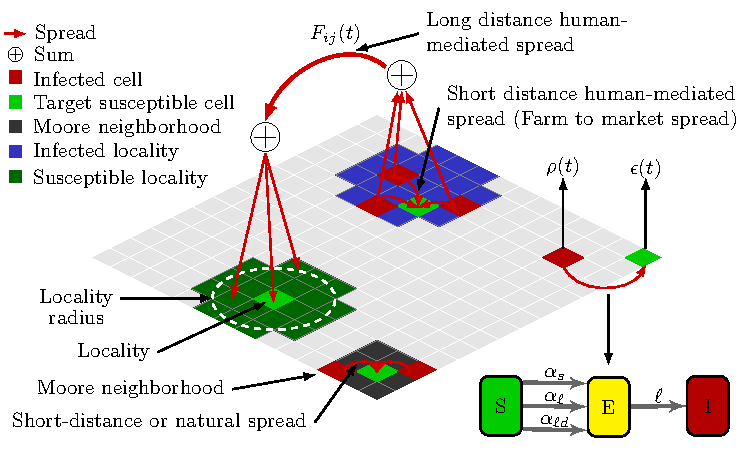
\includegraphics[width=1.1\textwidth]{figs/model_schematic.pdf}
\caption{\textbf{Multi-scale model of invasive species spread.} (a)~The
network structure, pathways and dynamics are captured in the illustration.
Also shown are the states and factors that influence state transitions:
infectiousness of a neighbor, suitability of the cell for pest
establishment, pathway parameters and latency period.
\label{fig:modelConcept}}
\end{figure}
%%
\begin{figure*}[!t]
\centering
\begin{subfigure}[b]{.32\textwidth}
    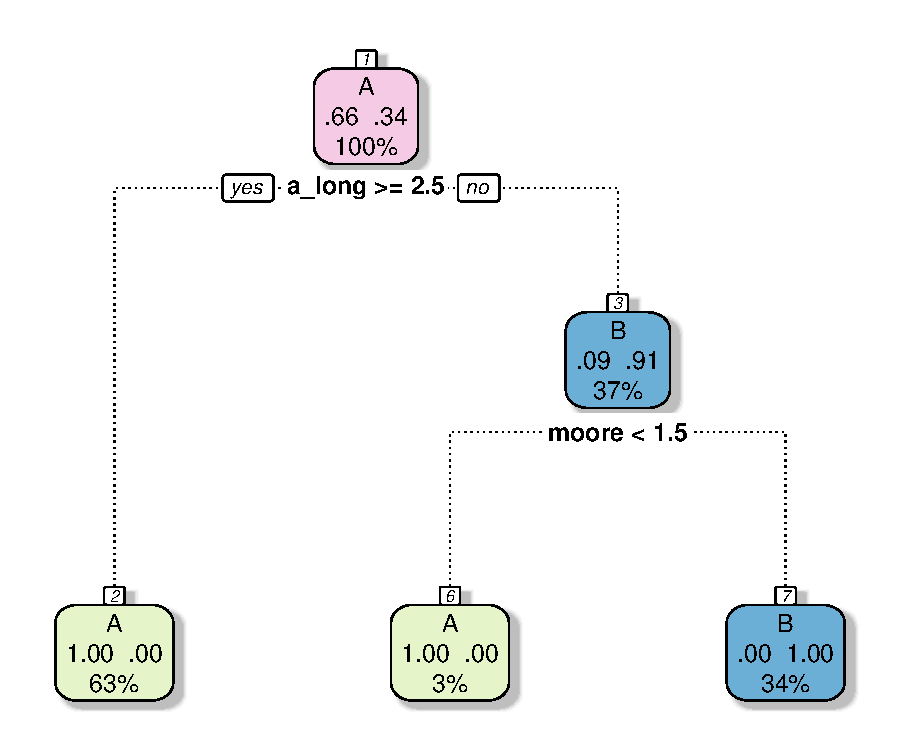
\includegraphics[width=\textwidth,trim=.6cm .6cm .6cm .6cm,clip]{../clustering/results/agglomerative/cart_cAB_agg.pdf}
\caption{$k=2$}
\end{subfigure}
\begin{subfigure}[b]{.32\textwidth}
    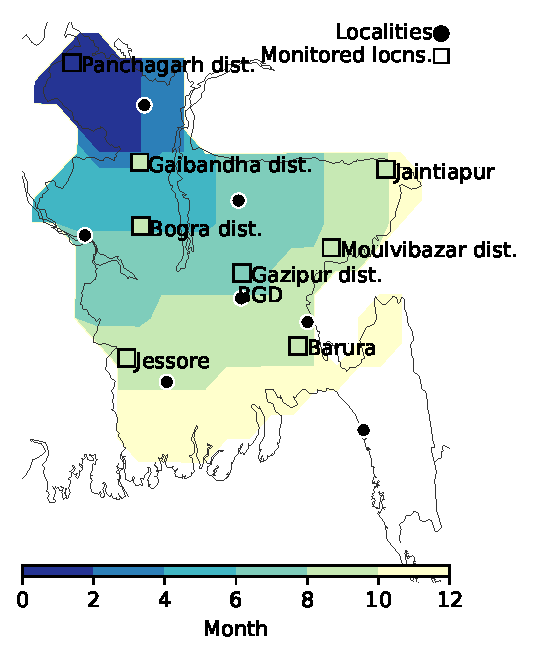
\includegraphics[width=\textwidth]{../cellular_automata/results/contour/BGD_model-A.pdf}
    \caption{Cluster~A \label{fig:bgdClassA}}
\end{subfigure}\hspace{.25cm}
\begin{subfigure}[b]{.32\textwidth}
    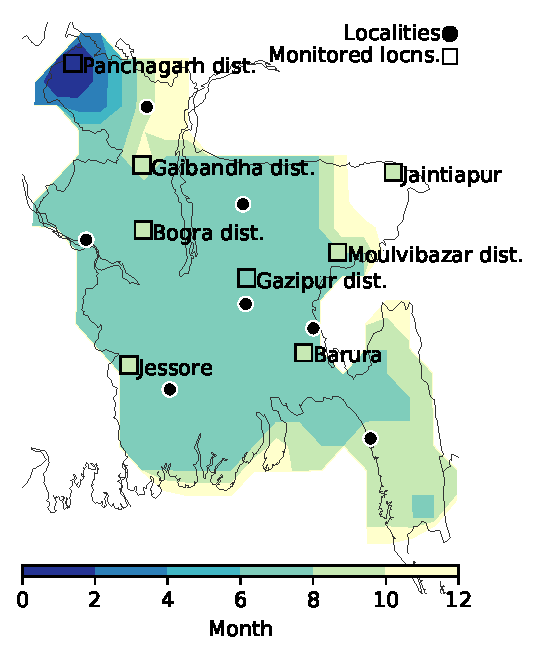
\includegraphics[width=\textwidth]{../cellular_automata/results/contour/BGD_model-B_m1_l3.pdf}
    \caption{Cluster~B \label{fig:bgdClassB1}}
\end{subfigure}
\caption{\textbf{Differenc.}The contour plots show the simulated
spread starting from the location of first report in Panchagarh district
for 12 months. For the purpose of plotting, the time of infection for a
cell is the minimum time step~$t$ such that the empirical probability that
the cell is infected by time~$t$ is $\ge0.8$. Also highlighted are the
eight monitored locations and the localities applied in the model. The
colors of the monitored locations correspond to the month of report
relative to the first report (Panchagarh). Two distinct spread patterns
emerged from the cluster analysis. (a) and (b) show representative spreads
observed for each class.}
\end{figure*}

\section{Related work}
state of the art and emerging trends
MAPSPAM

lamperti stuff one paragraph

%%
\section{Conclusion}

\bibliographystyle{named}
\bibliography{refs}
%%
\end{document}

